\section{Fraktální dimenze}\label{sec:fraktalni_dimenze}

\subsection{Chápání konceptu dimenze}\label{subsec:koncept-dimenze}

Výčet útvarů v sekci \ref{sec:sobepodobnost} splňoval zásadní vlastnost, a to sice, že všechny z nich byly \emph{soběpodobné}. V eukleidovské geometrii lze však u mnohých základních objektů pozorovat stejnou vlastnost. Např. čtverec lze určitě prohlásit v jistém smyslu za soběpodobný, neboť jej lze rozdělit na podobné útvary (viz obrázek \ref{fig:sobepodobnost-ctverce}).
\begin{figure}[h]
    \centering
    \begin{subfigure}[b]{\subfigwidth}
        \centering
        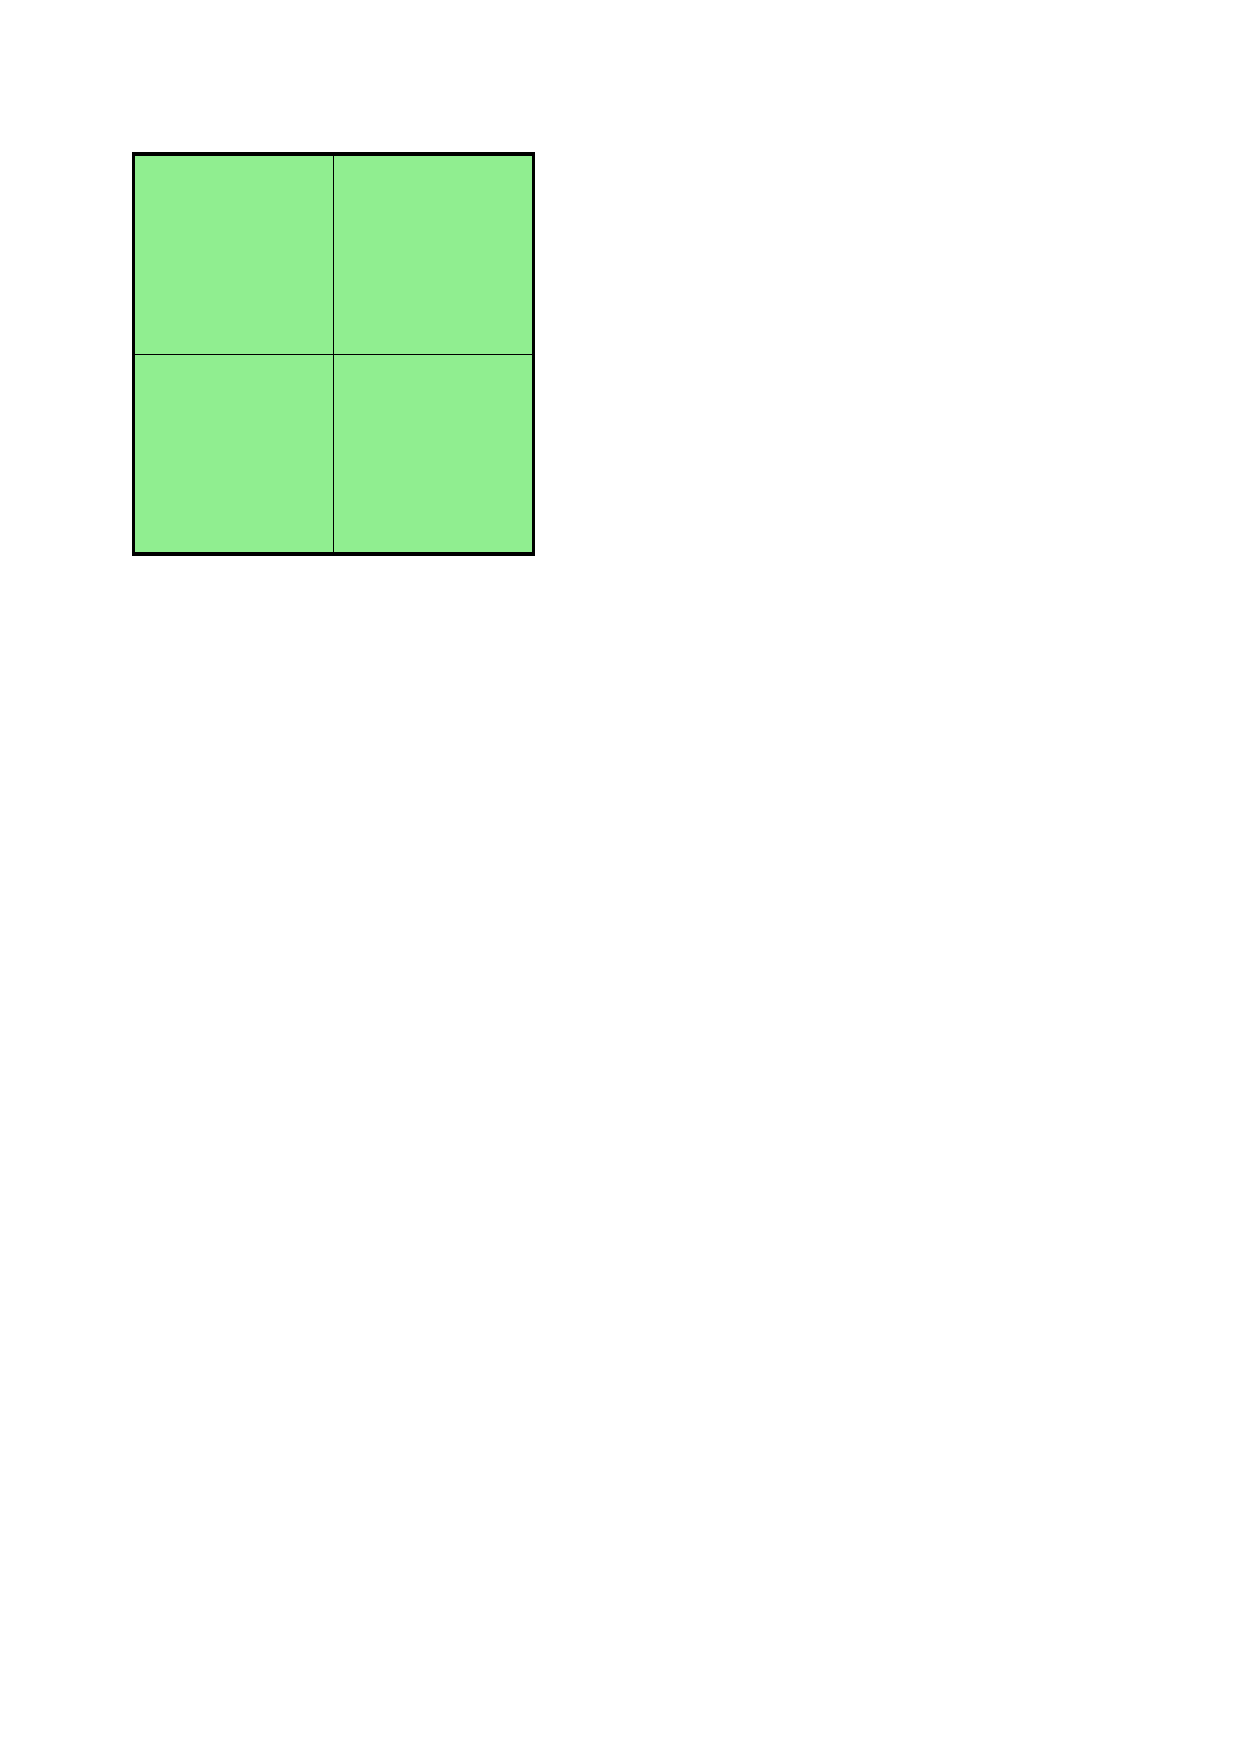
\includegraphics[scale=\normalipe]{ch01_ctverec_sobepodobnost.pdf}
        \caption{Čtverec rozdělený na čtyři menší čtverce.}
        \label{subfig:sobepodobnost-ctverce-1}
    \end{subfigure}
    \begin{subfigure}[b]{\subfigwidth}
        \centering
        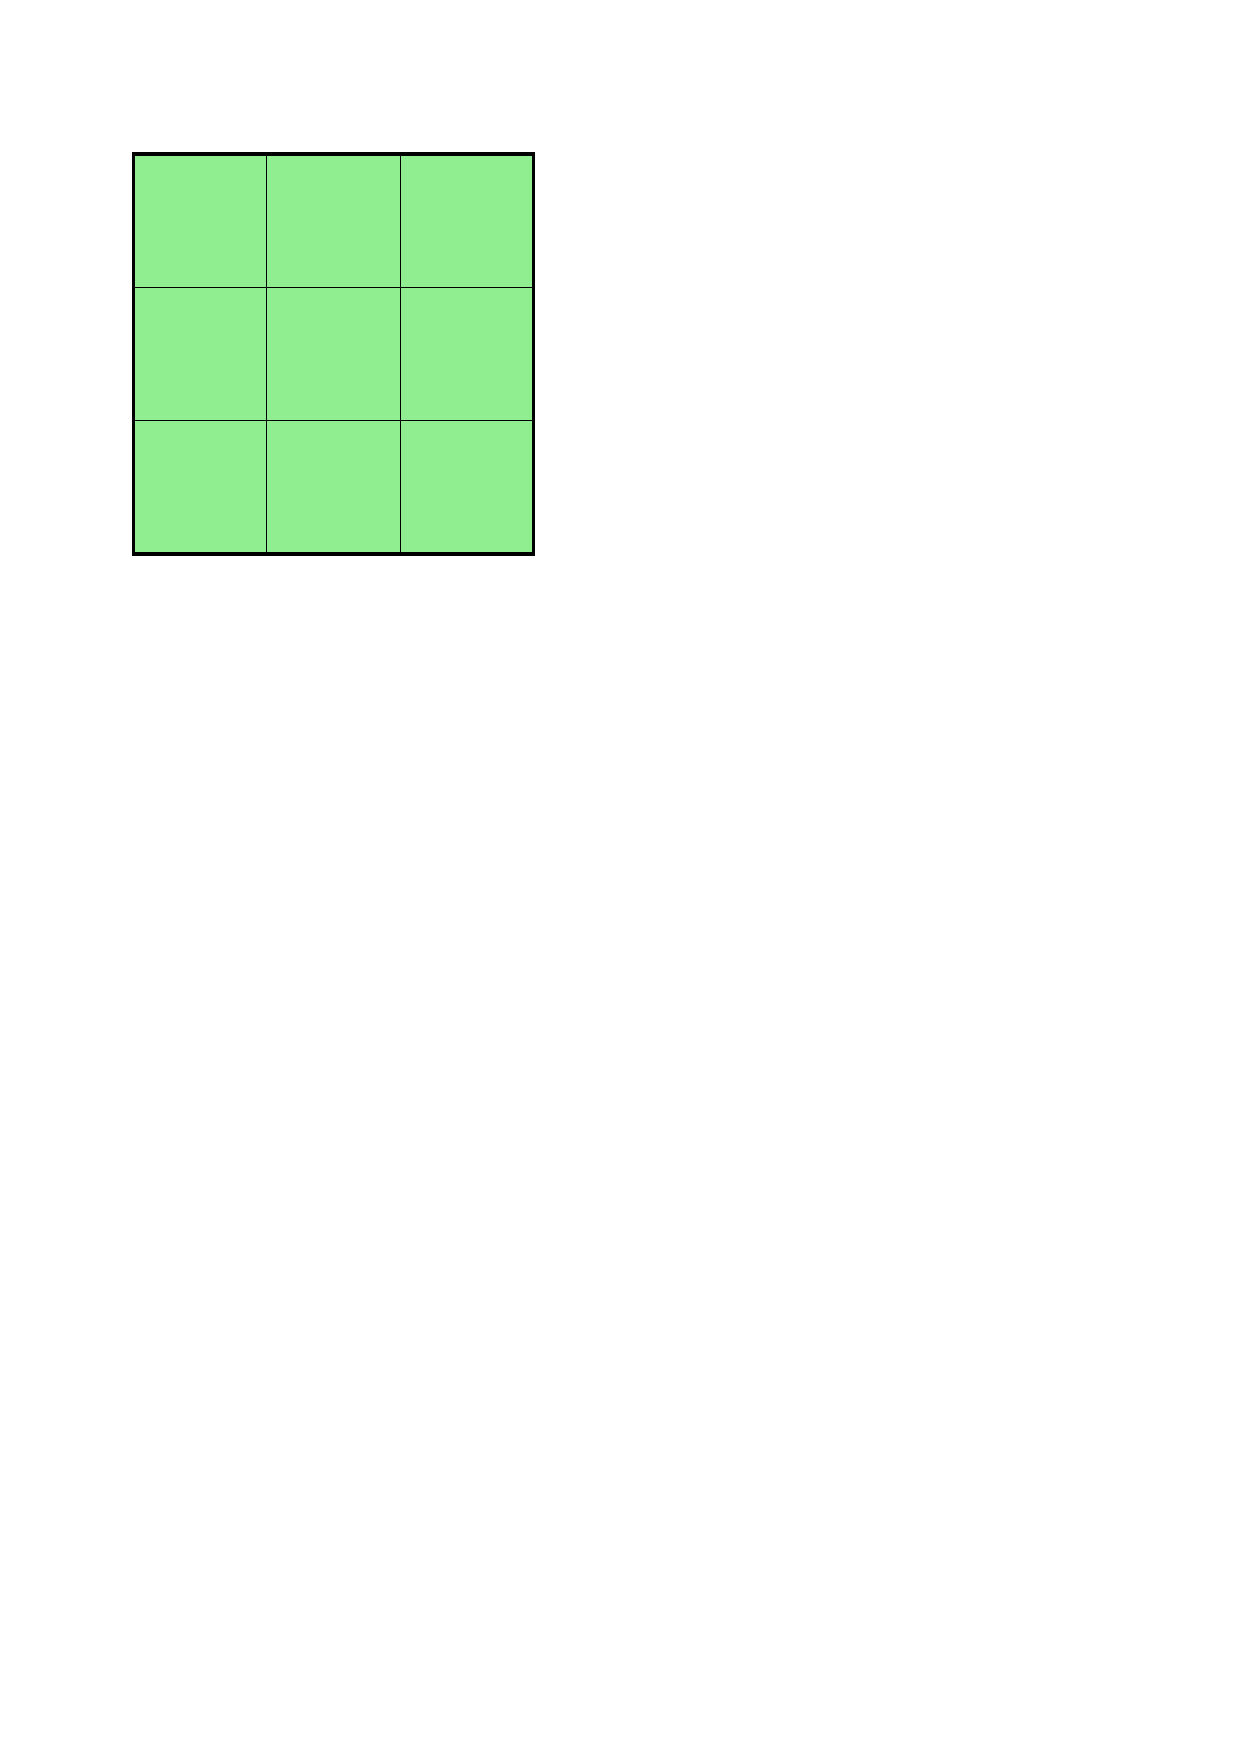
\includegraphics[scale=\normalipe]{ch01_ctverec_sobepodobnost_2.pdf}
        \caption{Jiná možnost rozdělení čtverce.}
        \label{subfig:sobepodobnost-ctverce-2}
    \end{subfigure}
    \caption{Soběpodobnost čtverce.}
    \label{fig:sobepodobnost-ctverce}
\end{figure}
Podobně např. i obyčejná úsečka je taktéž soběpodobná, protože ji můžeme rozdělit na obecně $k$ stejných částí (viz obrázek).\par
\begin{figure}[h]
    \centering
    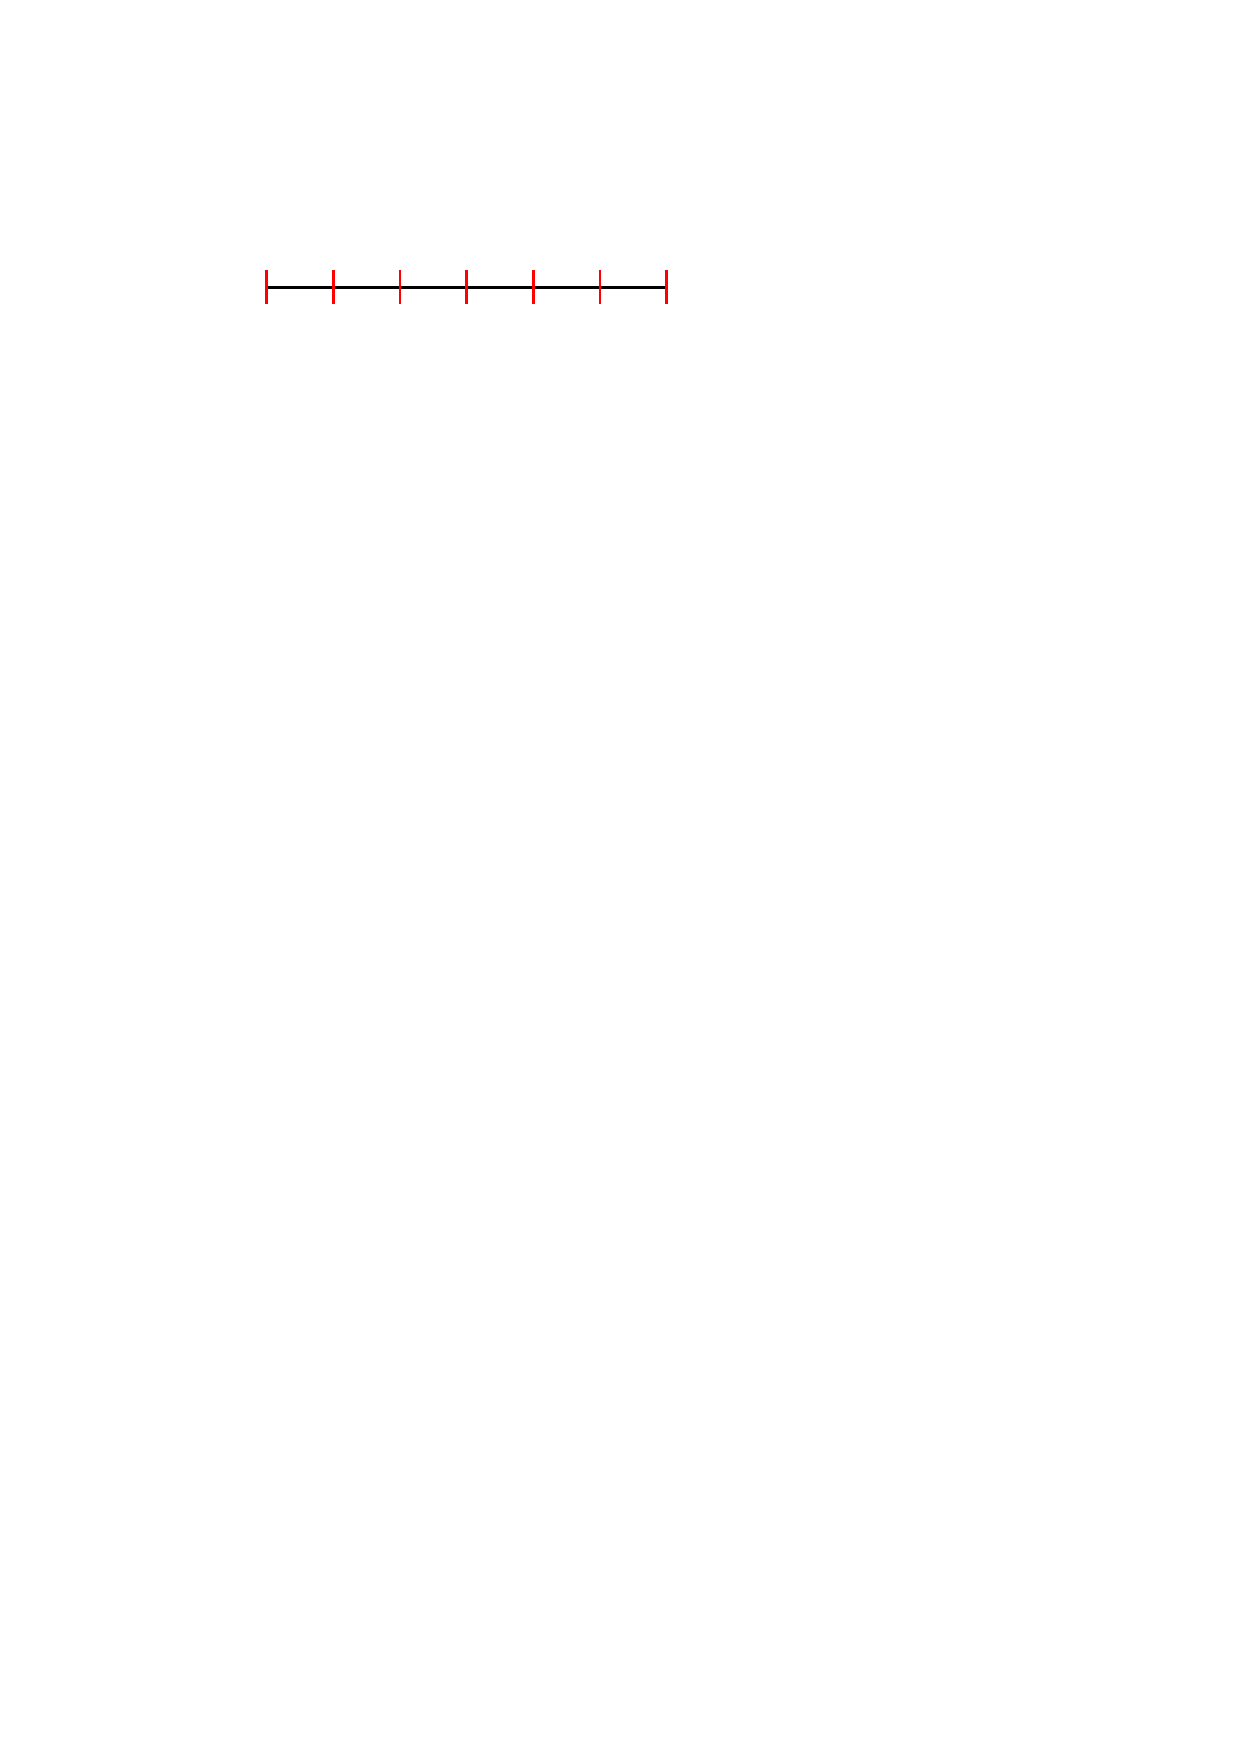
\includegraphics[scale=\normalipe]{ch01_usecka_sobepodobnost.pdf}
    \caption{Úsečka rozdělená na šest stejných částí.}
\end{figure}
K čemu nám takové uvědomnění vlastně je? Zmenšíme-li úsečku $k$-krát, pak budeme potřebovat přesně $k$ těchto částí, abychom dostali úsečku původní délky. U čtverce (nebo obdélkuníku obecně) při změnšení délky strany $k$-krát budeme potřebovat $k^2$ daných útvarů pro obdržení čtverce s původním obsahem.\footnote{Obdélník změnšený $k$-krát bude mít strany délek $a/k,\,b/k$, tedy jeho obsah bude
\[\dfrac{ab}{k^2}=\dfrac{S}{k^2},\]
kde $S$ je obsah původního obdélníka.}
Pro krychli bude situace zcela analogická, $k$-krát zmenšená kopie bude potřeba $k^3$-krát, abychom dostali krychli o původním objemu (viz obrázek \ref{fig:krychle-sobepodobnost}).
\begin{figure}[h]
    \centering
    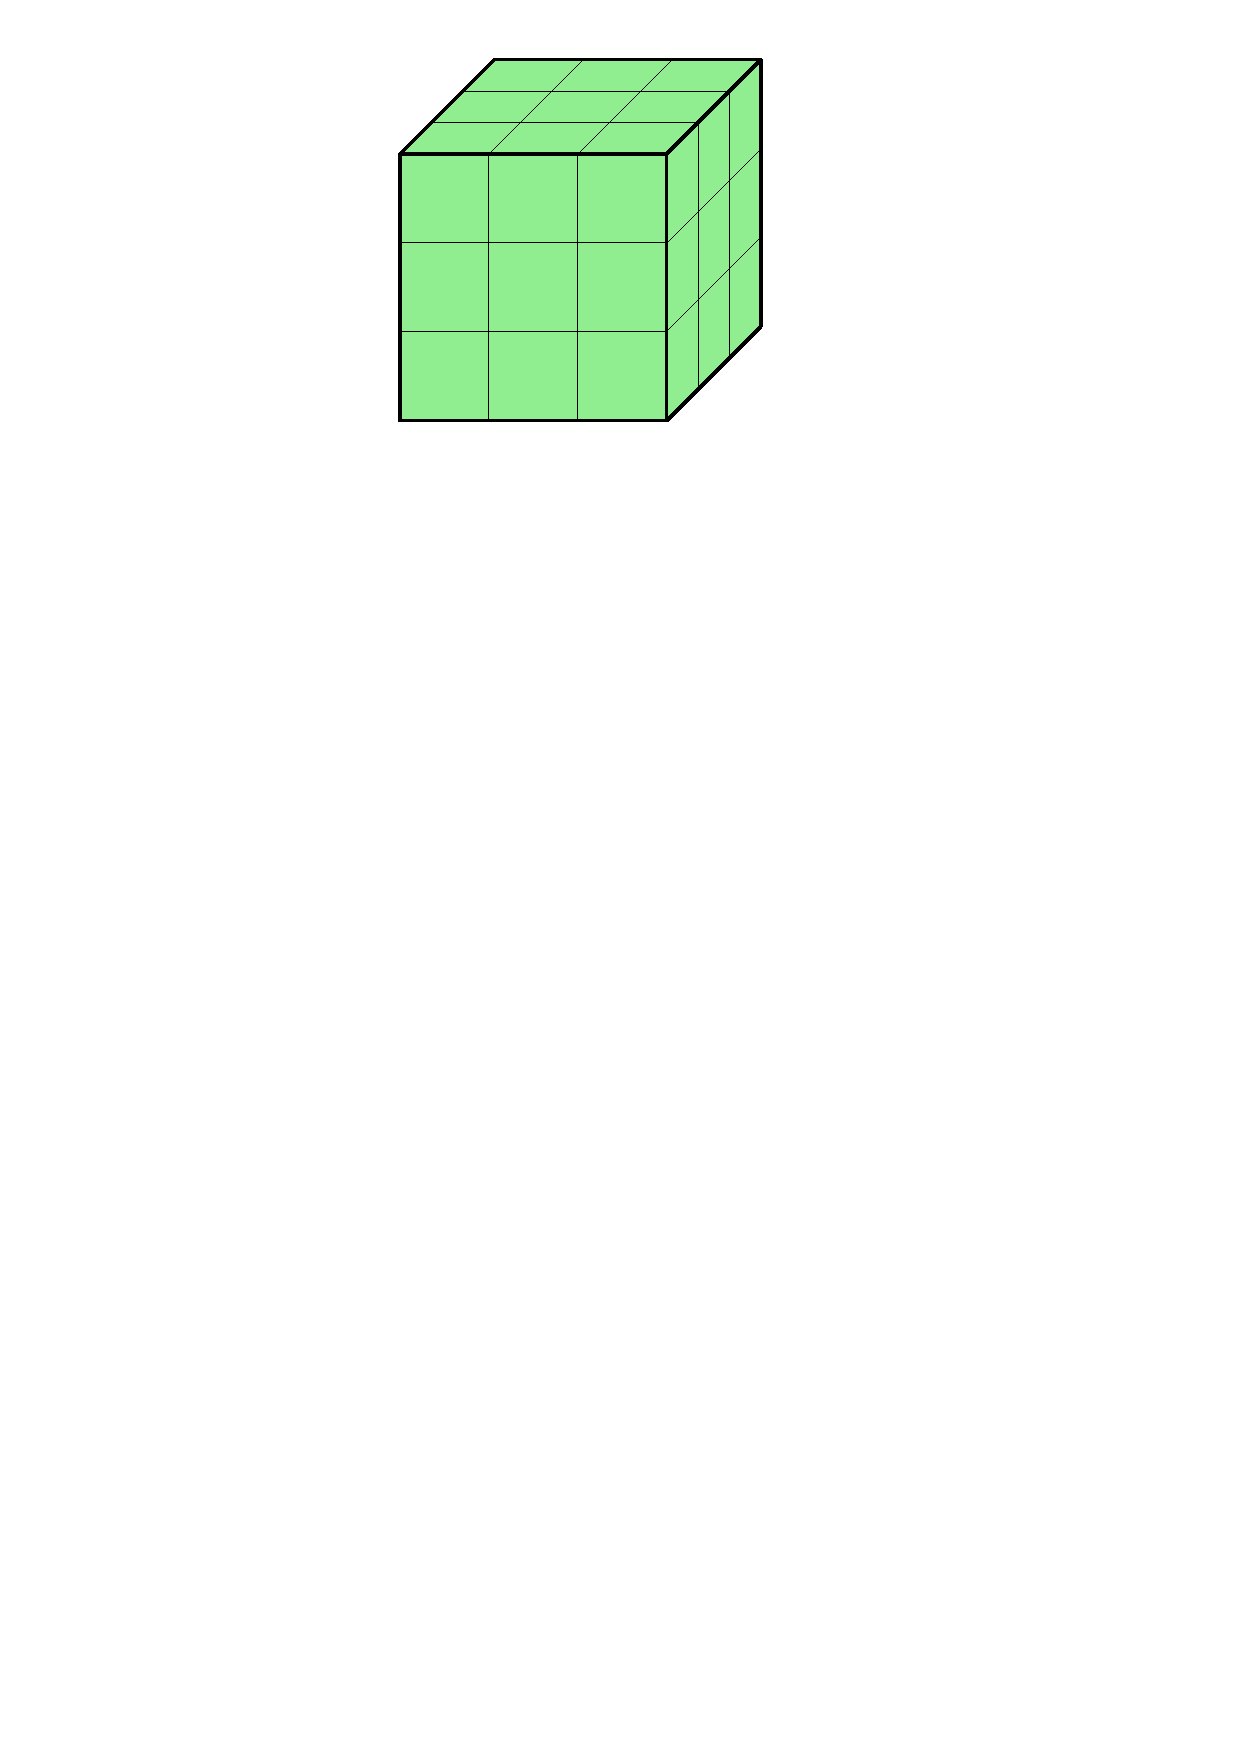
\includegraphics[scale=\normalipe]{ch01_krychle_sobepodobnost.pdf}
    \caption{Krychle rozdělená na 27 stejných částí.}
    \label{fig:krychle-sobepodobnost}
\end{figure}
Lze si všimnout, že v závislosti na \emph{dimenzi} objektu se mění daný exponent. Vztah lze tak zobecnit na
\begin{equation}\label{eq:pocet-utvaru}
    N(k)=k^d
\end{equation}
kde $N(k)$ je počet nových útvarů v závislosti na faktoru $k$ a $d$ je dimenze.\par
Čtenář si již nyní může všimnout, že toto je jeden z možných způsobů, jak lze chápat koncept dimenze. Jednoduchou úpravou rovnosti \eqref{eq:pocet-utvaru} dostaneme
\[d=\log_k{N(k)}=\dfrac{\ln{N(k)}}{\ln{k}}.\]
(Obecně lze volit jakýkoliv přípustný základ logaritmů, tj $d=\log_b{N(k)}/\log_b{k}$ pro $b\in\R^+\setminus\set{1}$.)
\begin{table}[h]
    \centering
    \begin{tabular}{r|cc}
    Útvar    & $N(k)$ & $d=\log_3{N(k)}/\log_3{k}$ \\ \hline
    Úsečka   & $3$      & $1$                          \\
    Čtverec  & $9$      & $2$                          \\
    Krychle  & $27$     & $3$                          \\
    Teserakt & $81$     & $4$                          \\
    \end{tabular}
    \label{table:eukleides-dimenze}
\end{table}
Dimenze v tomto pojetí skutečně dává dobrý smysl. Pro ``klasické'' geometrické objekty vychází dimenze vždy celočíselně.\par
Na této myšlence je založen pojem tzv. \emph{fraktální dimenze}\footnote{Někdy se též nazývá \emph{Kolmogorovova dimenze} nebo \emph{Hausdoffova-Besičovičova dimenze}. Je pojmenována po německém matematikovi \name{Felixi Hausdorffovi} (1869--1942) a ruských matematicích \name{Andreji Kolmogorovovi} (1903--1987) a \name{Abramovi Besičovičovi} (1891--1970).}. Existuje více způsobů její definice. Jeden z nich, kterého se dále budeme držet, je následující:
\begin{equation}\label{eq:fraktalni-dimenze}
    d_k=\lim_{\varepsilon\to 0^+}{\dfrac{\ln{N(\varepsilon)}}{\ln{\left(\dfrac{1}{\varepsilon}\right)}}}.
\end{equation}
(Převzato z \cite[str. 93]{Zelinka2006}.) Výraz $1/\varepsilon$ zde představuje faktor podobnosti jako původní $k$ (samotné $\varepsilon$ tak hraje roli měřítka), avšak největší rozdíl zde představuje zkoumání ``limitního chování'' daného výrazu.
\begin{example}[Fraktální dimenze úsečky]\label{ex:fraktalni-dimenze-usecka}
    Začněme asi nejednodušším příkladem výpočtu fraktální dimenze, a to u úsečky. Představme si, že úsečku \emph{jednotkové délky} rozdělíme na $N(\varepsilon)=n$ shodných dílů. Pak měřítko libovolného dílu je
    \[\varepsilon=\dfrac{1}{n}=n^{-1}.\]
    (Zde je dobré si uvědomit, že pro $n\to\infty$, tedy zjemňování dělení úsečky, platí, že $\varepsilon\to 0^+$.) Fraktální dimenzi úsečky vypočteme z definice jako
    \[d_k=\lim_{\varepsilon\to 0^+}{\dfrac{\ln{N(\varepsilon)}}{\ln{\left(\dfrac{1}{\varepsilon}\right)}}}=\lim_{n\to\infty}{\dfrac{\ln{n}}{\ln{n}}}=1.\]
\end{example}
\begin{example}[Fraktální dimenze čtverce]\label{ex:fraktalni-dimenze-ctverec}
    Podobně, jako v příkladu \ref{ex:fraktalni-dimenze-usecka} výše, můžeme stanovit i fraktální dimenzi čtverce. Uvažujme tedy čtverec o jednotkovém obsahu, který rozdělíme $N(\varepsilon)=n$ shodných útvarů. Přitom víme, že obsah mění kvadraticky vůči délce strany. Měřítko nového čtverce tak bude
    \[\varepsilon=\sqrt{\dfrac{1}{n}}=n^{-1/2}\]
    a fraktální dimenze vychází
    \[d_k=\lim_{n\to\infty}{\dfrac{\ln{n}}{\ln{n^{1/2}}}}=\lim_{n\to\infty}{\dfrac{\ln{n}}{\dfrac{1}{2}\ln{n}}}=2.\]
\end{example}
Pro krychli bude výpočet naprosto analogický (viz příklad \ref{ex:fraktalni-dimenze-ctverec}). Obecně pro $d$-rozměrnou krychli bude její fraktální dimenze\footnote{Obdobnou úvahou dojmeme k měřítku $\varepsilon=n^{-1/d}$.} rovna $d$.\par
Zkusme se nyní odprostit od krychle k trochu jinému útvaru.
\begin{example}[Fraktální dimenze trojúhelníku]\label{ex:fraktalni-dimenze-trojuhelnik}
    Podívejme se, jak to dopadne s fraktální dimenzí \emph{obecného trojúhelníku}. Každý trojúhelník $T$ lze rozdělit na čtveřici \emph{vzájemně shodných trojúhelníků $T_1,\dots,T_4$}, které vzniknou sestrojením středních příček v původním trojúhelníku (viz obrázek \ref{fig:trojuhelnik-sobepodobnost}).
    \begin{figure}[h]
        \centering
        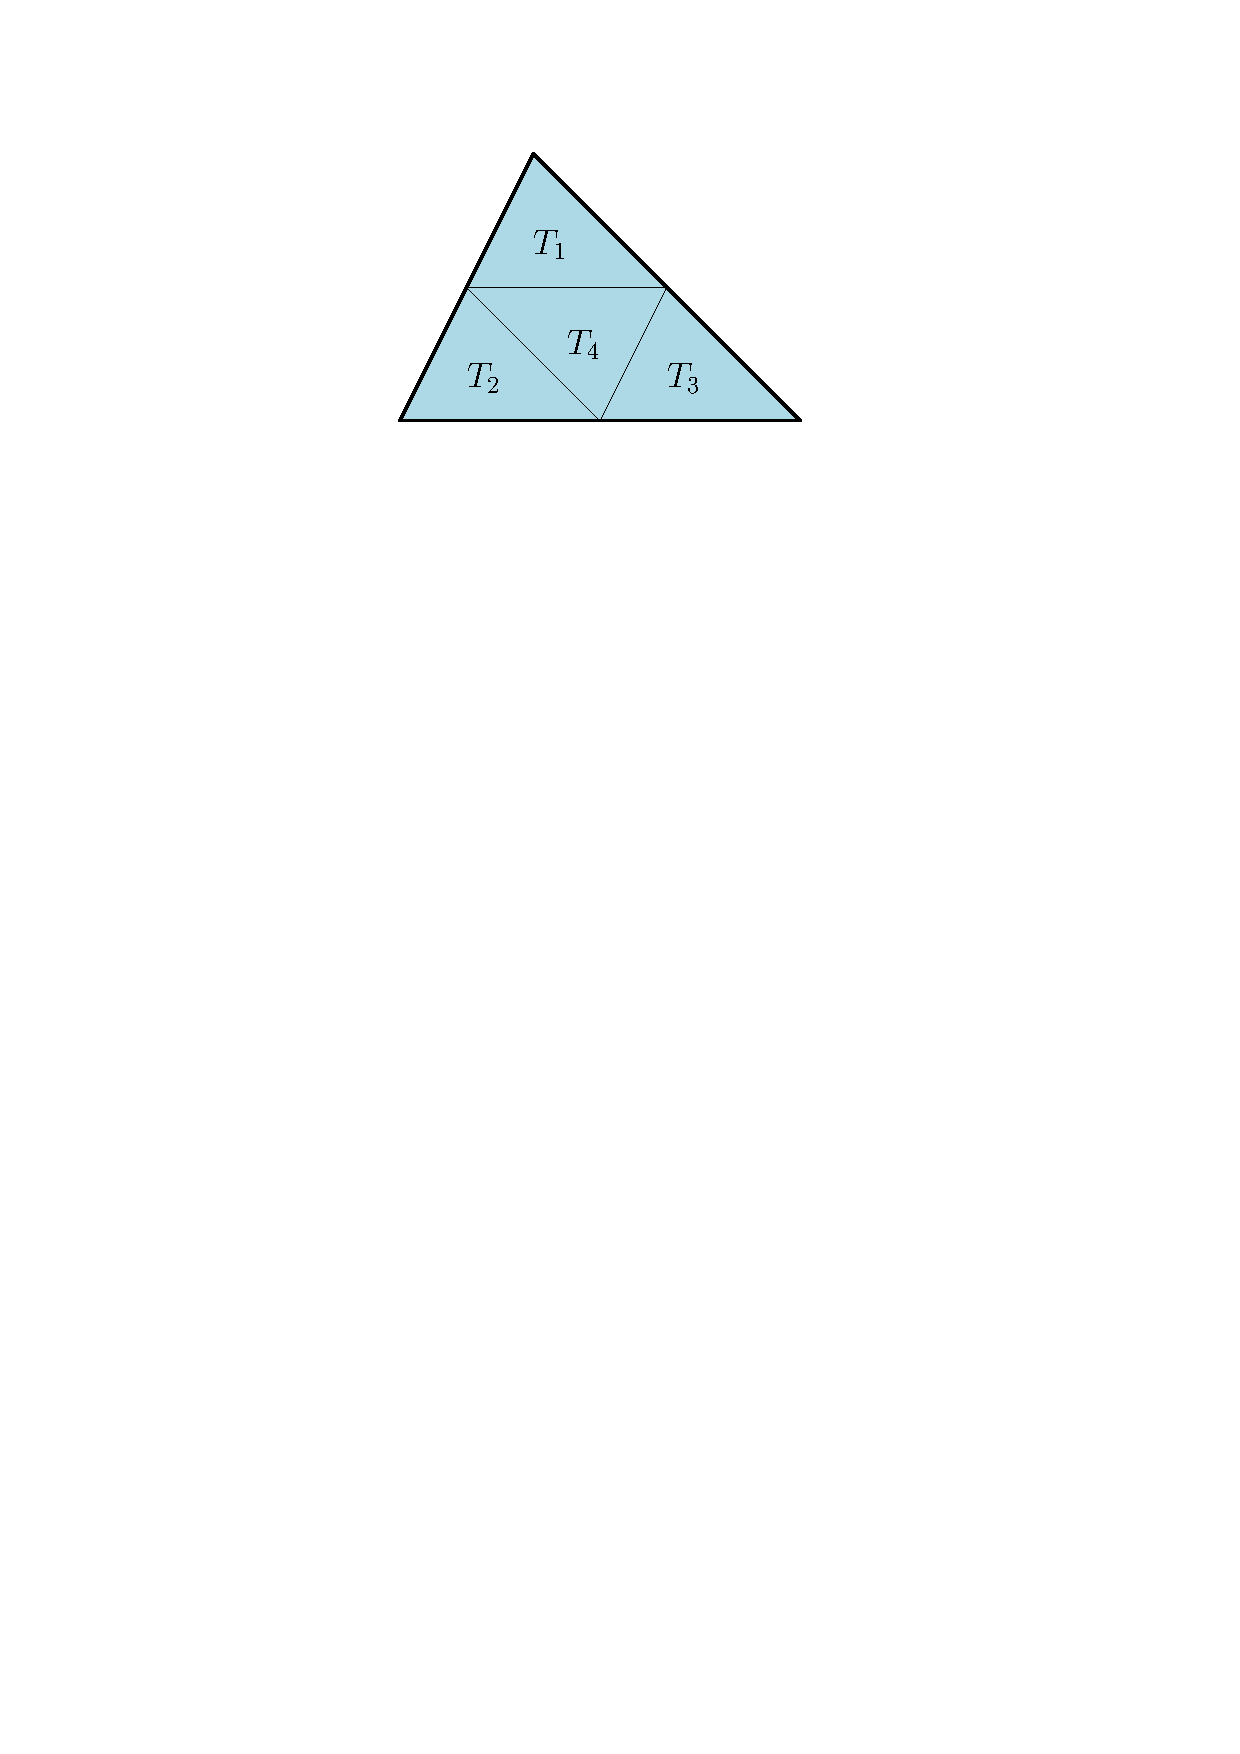
\includegraphics[scale=\normalipe]{ch01_trojuhelnik_sobepodobnost.pdf}
        \caption{Trojúhelník $T$ rozdělený na trojúhelníky $T_1,\dots,T_4$.}
        \label{fig:trojuhelnik-sobepodobnost}
    \end{figure}
    Délka každé střední příčky odpovídá polovině délky strany, s níž je rovnoběžná, tedy obsah každého z nich je \emph{čtvrtina obsahu původního} trojúhelníku $T$. Pokud obecně trojúhelník $T$ rozdělíme\footnote{Výpočet bychom mohli i zde provést ve stejném duchu jako u úsečky, čtverce nebo krychle. Počet částí, na než rozdělíme trojúhelník, označíme $N(\varepsilon)=n$, přičemž měřítko pak bude $\varepsilon=n^{-1/2}$.} takto na obecně $N(\varepsilon)=4^n$ pro nějaké $n\in\N$ shodných částí, pak měřítko každé z nich bude $\varepsilon=(1/2)^n$. Fraktální dimenze tak výchází:
    \[d_k=\lim_{n\to\infty}{\dfrac{\ln{4^n}}{\ln{2^n}}}=\lim_{n\to\infty}{\dfrac{2n\ln{2}}{n\ln{2}}}=2.\]
\end{example}

\subsection{Dimenze fraktálů}\label{subsec:dimenze-fraktalu}

Co kdybychom však zkusili podobnou myšlenku aplikovat i na \emph{fraktální objekty}? Zkusme to. Pro připomenutí jednotlivých křivek a výsledků k nim si dovoluji čtenáře opětovně odkázat na sekci \ref{sec:sobepodobnost}, kde jsou podrobněji rozebrány.
\begin{itemize}
    \item \textbf{Kochova křivka.} V každé iteraci nahrazujeme každou úsečku čtyřmi novými. Kompletní Kochova křivka tak obsahuje právě \emph{čtyři} kopie sebe sama zmenšených na třetinu, tj. v $n$-té iteraci je $N(\varepsilon)=4^n$, jak jsme již odvodili (viz podsekce \ref{subsec:kochova_krivka}).\footnote{Lze však zvolit i jiné dělení. Např. lze na Kochovu křivku nahlížet, že obsahuje \emph{16 kopií} sebe sama zmenšených na \emph{devítinu}.} Měřítko nové křivky je tak $\varepsilon=(1/3)^n$.
    \begin{equation}\label{eq:kochova-krivka-dimenze}
        d_k=\lim_{\varepsilon\to 0^+}{\dfrac{\ln{N(\varepsilon)}}{\ln{\left(\dfrac{1}{\varepsilon}\right)}}}=\lim_{n\to\infty}{\dfrac{\ln{4^n}}{\ln{3^n}}}=\dfrac{\ln{4}}{\ln{3}}\approx 1{,}2618595\dots
    \end{equation}
    \item \textbf{Kochova vločka.} Začínáme s rovnostranným trojúhelníkem o straně délky $1$, na jehož stranách postupně vznikne Kochova křivka. V $n$-té iteraci je obvod Kochovy vločky $o_n$ roven $3\cdot 4^n$, tj. i $N(\varepsilon)=3\cdot 4^n$, kde měřítko\footnote{Měřítko se ve srovnání s Kochovou křivkou liší v mocnině, neboť délku nových úseků porovnáváme s obvodem celého trojúhelníku, nikoliv pouze délkou jedné jeho strany. Nicméně ve výpočtu bych se mohli omezit i jen na jednu ze stran, výpočet by byl tak zcela identický, jako u Kochovy křivky.} nově vzniklých úseček je $\varepsilon=1/3\cdot(1/3)^n=(1/3)^{n+1}$. Není těžké se přesvědčit, že fraktální dimenze vychází stejně, jako u Kochovy křivky:
    \begin{equation}\label{eq:kochova-vlocka-dimenze}
        d_k=\lim_{n\to\infty}{\dfrac{\ln{3\cdot 4^n}}{\ln{3^{n+1}}}}=\dfrac{\ln{4^n}\overbrace{\left(1+\dfrac{\ln{3}}{\ln{4^n}}\right)}^{\to 1}}{\ln{3^n}\underbrace{\left(1+\dfrac{\ln{3}}{\ln{3^n}}\right)}_{\to 1}}=\dfrac{\ln{4}}{\ln{3}}
    \end{equation}
    \item \textbf{Sierpińského trojúhelník.} V každé iteraci vynecháme prostřední trojúhelník, čímž vznikne \emph{trojice} nových trojúhelníků s \emph{polovičním} měřítkem. Tzn. $N(\varepsilon)=3^n$ pro $\varepsilon=(1/2)^n$, a tedy
    \begin{equation}\label{eq:sierpinskeho-trojuhelnik-dimenze}
        d_k=\lim_{n\to\infty}{\dfrac{\ln{3^n}}{\ln{2^{n}}}}=\dfrac{\ln{3}}{\ln{2}}\approx 1{,}5849625\dots
    \end{equation}
    \item \textbf{Cantorovo diskontinuum.} Vždy vyjmeme prostřední třetinu úsečky, čímž obdržíme \emph{dvojici} úseček \emph{třetinové} délky, tj. $N(\varepsilon)=2^n$ pro $\varepsilon=(1/3)^n$. Fraktální dimenze tak vychází
    \begin{equation}\label{eq:cantorovo-diskontinuum-dimenze}
        d_k=\lim_{n\to\infty}{\dfrac{\ln{2^n}}{\ln{3^n}}}=\dfrac{\ln{2}}{\ln{3}}\approx 0{,}6309297\dots
    \end{equation}
\end{itemize}
Udělejme si nyní menší souhrn a porovnání dosavadně získaných výsledků (viz tabulka \ref{table:fraktaly-eukleides-dimenze}).
\begin{table}[h]
    \centering
    \begin{tabular}{r|ccc}
        Útvar                    & $\varepsilon$ & $N(\varepsilon)$ & $d_k$              \\ \hline
        Úsečka                   & $n^{-1}$      & $n$              & 1                  \\
        Čtverec                  & $n^{-1/2}$    & $n$              & 2                  \\
        Krychle                  & $n^{-1/3}$    & $n$              & 3                  \\
        Teserakt                 & $n^{-1/4}$    & $n$              & 4                  \\
        $d$-rozměrná krychle     & $n^{-1/d}$    & $n$              & $d$                \\
        Obecný trojúhelník       & $(1/2)^n$     & $4^n$            & 2                  \\
        Kochova křivka           & $(1/3)^n$     & $4^n$            & $1{,}2618595\dots$ \\
        Kochova vločka           & $(1/3)^{n+1}$ & $3\cdot 4^n$     & $1{,}2618595\dots$ \\
        Sierpińského trojúhelník & $(1/2)^n$     & $3^n$            & $1{,}5849625\dots$ \\
        Cantorovo diskontinuum   & $(1/3)^n$     & $2^n$            & $0{,}6309297\dots$ \\
    \end{tabular}
    \caption{Porovnání fraktálních dimenzí $d_k$ různých objektů.}
    \label{table:fraktaly-eukleides-dimenze}
\end{table}
Můžeme si všimnout, že zatímco u ``klasických'' objektů vychází fraktální dimenze \emph{celočíselná}, u fraktálů vychází \emph{neceločíselně}, ba dokonce i iracionálně.